%%
%% Copyright 2007-2019 Elsevier Ltd
%%
%% This file is part of the 'Elsarticle Bundle'.
%% ---------------------------------------------
%%
%% It may be distributed under the conditions of the LaTeX Project Public
%% License, either version 1.2 of this license or (at your option) any
%% later version.  The latest version of this license is in
%%    http://www.latex-project.org/lppl.txt
%% and version 1.2 or later is part of all distributions of LaTeX
%% version 1999/12/01 or later.
%%
%% The list of all files belonging to the 'Elsarticle Bundle' is
%% given in the file `manifest.txt'.
%%
%% Template article for Elsevier's document class `elsarticle'
%% with harvard style bibliographic references

%\documentclass[preprint,12pt]{elsarticle}

%\textheight 230mm \textwidth 170mm \topmargin 0.5cm \oddsidemargin
%0pt \evensidemargin 0pt
%\parskip=2mm
%\voffset -2cm
%% Use the option review to obtain double line spacing
%\documentclass[preprint,review,12pt]{elsarticle}

%% Use the options 1p,twocolumn; 3p; 3p,twocolumn; 5p; or 5p,twocolumn
%% for a journal layout:
%\documentclass[final,1p,times]{elsarticle}
 %\documentclass[final,1p,times,twocolumn]{elsarticle}
\documentclass[final,3p,times]{elsarticle}
%% \documentclass[final,3p,times,twocolumn]{elsarticle}
%% \documentclass[final,5p,times]{elsarticle}
%% \documentclass[final,5p,times,twocolumn]{elsarticle}

%% For including figures, graphicx.sty has been loaded in
%% elsarticle.cls. If you prefer to use the old commands
%% please give \usepackage{epsfig}

%% The amssymb package provides various useful mathematical symbols
\usepackage{amssymb}
\usepackage{graphicx,setspace}
\usepackage{psfrag}
\usepackage{amsfonts}
\expandafter\let\csname equation*\endcsname\relax
\expandafter\let\csname endequation*\endcsname\relax
\usepackage{amsmath}
\usepackage{amssymb, amsthm}
\usepackage{mathrsfs}
\usepackage{epstopdf}
\usepackage{float}
\usepackage{lineno,hyperref}
\usepackage{color}
\usepackage{subfigure}

\usepackage{amsmath}
%\usepackage{amsthm}
\usepackage{dsfont} % it is the package of using the "\mathds{} "
\usepackage{amssymb} % it is the package of using the "\mathbb{}"
\usepackage{graphicx,color}
\usepackage{extarrows}

\bibliographystyle{elsarticle-num}
\usepackage{graphicx}

\usepackage{epstopdf}
%% The amsthm package provides extended theorem environments
%% \usepackage{amsthm}

%% The lineno packages adds line numbers. Start line numbering with
%% \begin{linenumbers}, end it with \end{linenumbers}. Or switch it on
%% for the whole article with \linenumbers.
%% \usepackage{lineno}

\journal{?}

\begin{document}
\newtheorem{definition}{Definition}[section]
\newtheorem{lemma}{Lemma}[section]
\newtheorem{remark}{Remark}[section]
\newtheorem{theorem}{Theorem}[section]
\newtheorem{proposition}{Proposition}
\newtheorem{assumption}{Assumption}
\newtheorem{example}{Example}
\newtheorem{corollary}{Corollary}[section]
\def\ep{\varepsilon}
\def\Rn{\mathbb{R}^{n}}
\def\Rm{\mathbb{R}^{m}}
\def\E{\mathbb{E}}
\def\hte{\hat\theta}
%\numberwithin{theorem}{section}
%\numberwithin{definition}{section}
\renewcommand{\theequation}{\thesection.\arabic{equation}}
\begin{frontmatter}

%% Title, authors and addresses

%% use the tnoteref command within \title for footnotes;
%% use the tnotetext command for theassociated footnote;
%% use the fnref command within \author or \address for footnotes;
%% use the fntext command for theassociated footnote;
%% use the corref command within \author for corresponding author footnotes;
%% use the cortext command for theassociated footnote;
%% use the ead command for the email address,
%% and the form \ead[url] for the home page:
%% \title{Title\tnoteref{label1}}
%% \tnotetext[label1]{}
%% \author{Name\corref{cor1}\fnref{label2}}
%% \ead{email address}
%% \ead[url]{home page}
%% \fntext[label2]{}
%% \cortext[cor1]{}
%% \address{Address\fnref{label3}}
%% \fntext[label3]{}




\title{Coupled Josephson junctions}


%% \author[label1,label2]{}
%% \address[label1]{}
%% \address[label2]{}

\author{Ruijie He\fnref{addr1,addr2}}\ead{gravitas_sysu@qq.com}
\author{Shenglan Yuan\corref{cor1}\fnref{addr1}}
\ead{shenglanyuan@gbu.edu.cn}\cortext[cor1]{Corresponding author}


\address[addr1]{\rm Department of Mathematics, School of Sciences, Great Bay University, Dongguan 523000, China }
\address[addr2]{\rm School of Mathematics,Sun Yat-sen University, Guangzhou 510275, China}








\begin{abstract}

\end{abstract}

\begin{keyword}

%% keywords here, in the form: keyword \sep keyword

%% PACS codes here, in the form: \PACS code \sep code

%% MSC codes here, in the form: \MSC code \sep code
%% or \MSC[2008] code \sep code (2000 is the default)

\end{keyword}

\end{frontmatter}

%% \linenumbers

%% main text
\section{Introduction}
The application of score-based generative models to Josephson junction systems offers several compelling advantages over traditional analytical methods. Unlike conventional approaches that require explicit equation solving under simplifying assumptions, this data-driven framework learns directly from observational or simulated data, capturing the intrinsic stochasticity and nonlinear coupling without mathematical approximations. The method naturally handles high-dimensional state spaces, scaling efficiently to complex multi-junction arrays where traditional techniques face exponential computational barriers. Its exceptional capability for rare event sampling enables the study of physically crucial but statistically improbable phenomena like quantum phase slips and switching events that would be computationally prohibitive to capture through direct simulation. Furthermore, the approach seamlessly incorporates experimental measurements directly into the learning process, bridging the gap between theoretical models and real-world device behavior. Finally, the probabilistic nature of generative models provides inherent uncertainty quantification, offering not just point estimates but full distributional information about junction states and parameters, which is essential for assessing the reliability and noise resilience of quantum circuits in practical applications.

This innovative approach promises to reveal profound insights into the collective dynamics of quantum circuits, uncovering novel synchronization patterns in junction arrays that transcend simple pairwise coupling and exhibit complex spatiotemporal ordering. By mapping the complete dynamical landscape, we can identify optimal coupling configurations that maximize coherence and minimize decoherence in quantum computing applications, potentially leading to more robust qubit designs and quantum memory elements. The framework naturally elucidates the noise resilience properties of different array geometries, demonstrating how specific topological arrangements can either amplify or suppress the impact of thermal fluctuations and environmental noise. Furthermore, scaling to large-scale systems enables the discovery of emergent collective phenomena--such as topological protection, many-body localization, and quantum synchronization transitions--that arise only in the thermodynamic limit and cannot be predicted from individual component behavior. The powerful combination of rigorous physical modeling, embodied in the coupled Josephson junction equations, with modern generative AI represents a transformative direction for investigating complex quantum systems, bridging the gap between microscopic physics and macroscopic emergent behavior while providing unprecedented predictive capabilities for designing next-generation quantum technologies.

\section{Coupled Josephson junction equations }
We consider a two-junction superconducting quantum interference device (SQUID).
The system consists of a superconducting loop interrupted by two Josephson junctions with the structure S-I-S-I-S. For multiple junctions, we have to consider the phases of each junction and the coupling between them. The phases across the junctions are denoted by $\phi_1$ and $\phi_2$. The external magnetic flux is set to zero for simplicity: $\Phi_{\text{ext}}=0$. The voltage across each junction is related to the phase by

\begin{equation}\label{Vj}
V_j=\frac{\hbar}{2e}\dot{\phi}_j,\quad \text{for}\,\,j=1,2.
\end{equation}

Using the resistively and capacitively shunted junction (RCSJ) model, the current through each junction is

\begin{equation}\label{Ij}
I_j=I_{c_j}\sin(\phi_j)+\frac{V_j}{R_j}+C_j\dot{V}_j,
\end{equation}

where $I_{c_j}$ are critical currents, $R_j$ represent resistances, and $C_j$ stand for capacitances.
Substituting \eqref{Vj} for $V_j$ into \eqref{Ij} yeilds

\begin{equation}\label{Ij2}
I_j=I_{c_j}\sin(\phi_j)+\frac{\hbar}{2eR_j}\dot{\phi}_j+\frac{\hbar C_j}{2e}\ddot{\phi}_j.
\end{equation}

In a SQUID, the total bias current $I$ splits as $I=I_1+I_2$. We can decompose the currents through junctions into symmetric and antisymmetric components:

\begin{equation}\label{I}
I_1=\frac{I}{2}+I_{\text{circ}},\quad I_2=\frac{I}{2}-I_{\text{circ}},
\end{equation}

where $I_{\text{circ}}$ means the circulating current around the loop.
The flux quantization condition with $\Phi_{\text{ext}}=0$ gives

\begin{equation*}
\phi_1-\phi_2=\frac{2e}{\hbar}LI_{\text{circ}},
\end{equation*}

where $L$ is the loop inductance. Thus,

\begin{equation}\label{CC}
I_{\text{circ}}=\frac{\hbar}{2eL}(\phi_1-\phi_2).
\end{equation}

Substitute~\eqref{Ij} and~\eqref{CC} into the expressions for $I_1$ and $I_2$

\begin{align}\label{I1}
\frac{I}{2}+\frac{\hbar}{2eL}(\phi_1-\phi_2)&=I_{c_1}\sin(\phi_1)+\frac{\hbar}{2eR_1}\dot{\phi}_1+\frac{\hbar C_1}{2e}\ddot{\phi}_1,\\ \label{I2}
  \frac{I}{2}-\frac{\hbar}{2eL}(\phi_1-\phi_2)&=I_{c_2}\sin(\phi_2)+\frac{\hbar}{2eR_2}\dot{\phi}_2+\frac{\hbar C_2}{2e}\ddot{\phi}_2.
\end{align}

We divide~\eqref{I1} by $I_{c_1}$, and thus get

\begin{equation*}
\frac{\hbar C_1}{2eI_{c_1}}\ddot{\phi}_1+\frac{\hbar}{2eR_1I_{c_1}}\dot{\phi}_1+\sin(\phi_1)
=\frac{I}{2I_{c_1}}+\frac{\hbar}{2eLI_{c_1}}(\phi_1-\phi_2).
\end{equation*}

We introduce normalized time $t=\omega_{p_1}\tau$, where the plasma frequency is
\begin{equation*}
\omega_{p_1}=\sqrt{\frac{2eI_{c_1}}{\hbar C_1}}.
\end{equation*}
Hence,
\begin{equation}\label{sI1}
\ddot{\phi}_1+\beta_{J_1}\dot{\phi}_1+\sin(\phi_1)
=i_1+\frac{\hbar}{2eLI_{c_1}}(\phi_1-\phi_2),
\end{equation}
where $\beta_{J_1}=\frac{1}{\omega_{p_1}R_1 C_1}$ and $i_1=\frac{I}{2I_{c_1}}$.
We define the coupling constant
\begin{equation*}
\kappa_1=-\frac{\hbar}{2eLI_{c_1}}.
\end{equation*}

So~\eqref{sI1} becomes

\begin{equation}\label{dI1}
\ddot{\phi}_1+\beta_{J_1}\dot{\phi}_1+\sin(\phi_1)
=i_1+\kappa_1(\phi_2-\phi_1),
\end{equation}

Similarly, we divide \eqref{I2} by $I_{c_2}$ and  normalize using $\omega_{p_2}=\sqrt{\frac{2eI_{c_2}}{\hbar C_2}}$:

\begin{equation}\label{sI2}
\ddot{\phi}_2+\beta_{J_2}\dot{\phi}_2+\sin(\phi_2)
=i_2-\frac{\hbar}{2eLI_{c_2}}(\phi_1-\phi_2).
\end{equation}

We define the coupling constant

\begin{equation*}
\kappa_2=-\frac{\hbar}{2eLI_{c_2}}.
\end{equation*}

Therefore,

\begin{equation}\label{dI2}
\ddot{\phi}_2+\beta_{J_2}\dot{\phi}_2+\sin(\phi_2)
=i_2+\kappa_2(\phi_1-\phi_2).
\end{equation}

According to the fluctuation-dissipation theorem, thermal noise currents $i_{\text{th}1}$ and $i_{\text{th}2}$
are added to the right-hand sides of~\eqref{dI1} and~\eqref{dI2}. These represent Johnson-Nyquist noise from the resistors.

Finally, the coupled Josephson junction equations are
\begin{align}\label{n1}
\ddot{\phi_1}+\beta_{J_1}\dot{\phi_1}+\sin \phi_1&=i_1+i_{\text{th}1}(t)+\kappa_1(\phi_2-\phi_1),  \\ \label{n2}
\ddot{\phi_2}+\beta_{J_2}\dot{\phi_2}+\sin \phi_2&=i_2+i_{\text{th}2}(t)+\kappa_2(\phi_1-\phi_2).
\end{align}


\section{Learning phase space dynamics }
Generative modeling by estimating gradients of the data distribution (also known as score-based generative models or diffusion models) is a powerful framework that could be very well-suited for investigating complex systems like coupled Josephson junctions.

The key idea is to learn the score function, i.e., the gradient of the log probability density
$\nabla_{\textbf{x}}\log p(\textbf{x})$, where for our junction system as in \eqref{n1}-\eqref{n2}, $\textbf{x}=[\phi_1,\phi_2,\dot{\phi}_1,\dot{\phi}_2]$ represents the state vector. We could train score-based models to capture the complex joint distribution of junction states. Instead of solving the coupled equations \eqref{n1}-\eqref{n2} directly, we
collect trajectory data from simulations, train a score-based model on the joint distribution of states and generate new trajectories that respect the underlying physics.

 The score function $\nabla\log p(\phi_1,\phi_2,\dot{\phi}_1,\dot{\phi}_2)$ would capture how likely the system is to transition between different dynamical regimes. It implicitly learn the coupling terms and thermal noise characteristics. The fluctuation-dissipation theorem relates thermal noise to damping. Score-based models could separate deterministic dynamics from stochastic components, characterize noise correlations between junctions and identify non-thermal noise sources.

\textbf{Implementation framework}
\begin{description}
  \item[Step 1] Data generation\\
  We simulate the coupled equations \eqref{n1}-\eqref{n2} with different parameter settings and initial conditions.
  \item[Step 2] Score network architecture\\
 We design a neural network that respects physical constraints:
 \begin{itemize}
   \item Periodicity in $\phi_1,\phi_2$ (mod $2\pi$)
   \item Time-translation invariance for stationary processes
   \item Potential symmetry between junctions
 \end{itemize}
  \item[Step 3] Training with denoising score matching\\
  We use the objective
  \begin{equation*}
  \mathbb{E}_{t,\textbf{x},\tilde{\textbf{x}}}[\lambda(t)\|s_\theta(\tilde{\textbf{x}},t)-\nabla_{\tilde{\textbf{x}}}\log p_{0t}(\tilde{\textbf{x}}|\textbf{x})\|],
  \end{equation*}
\end{description}
where $\tilde{\textbf{x}}$ is a noisy version of the true state $\textbf{x}$. The learned score function should reveal preferred phase difference configurations $(\phi_1-\phi_2)$.


\begin{figure}[H]
\begin{center}
\begin{minipage}{4in}
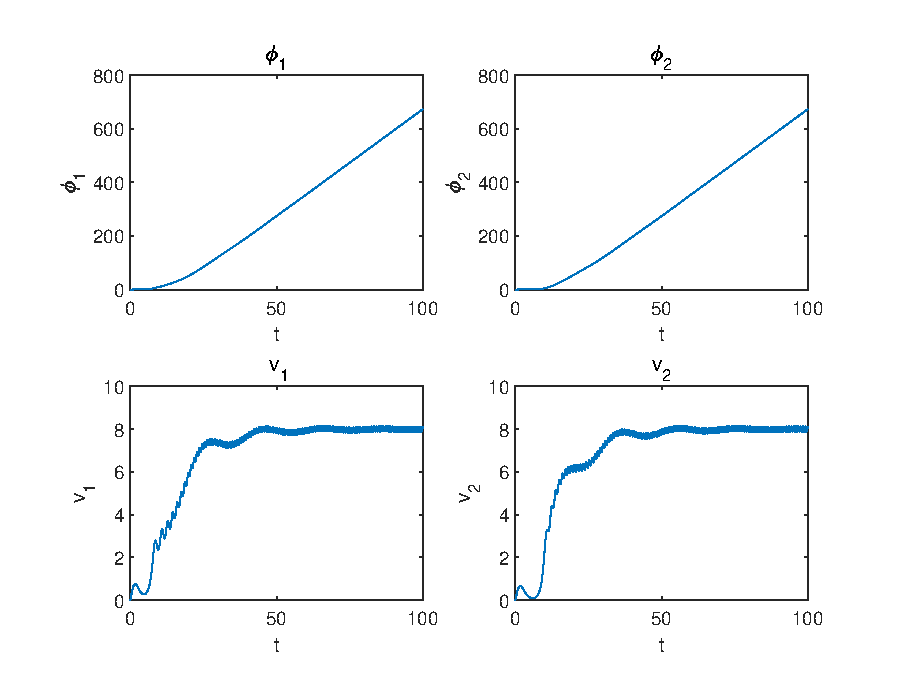
\includegraphics[width=4in]{CoupledJ.eps}
\end{minipage}
\end{center}
\caption{The coupled Josephson junction dynamics (without noise) for a given set of parameters: $\beta_{J_i}=0.1$, $i_{c_i}=0.8$, $\kappa_i=0.05$, $i=1, 2$.}
\end{figure}
Let $v_1=\dot{\phi}_1$ and $v_2=\dot{\phi}_2$. We can rewrite he following normalized equations \eqref{dI1} and \eqref{dI2} without noise as a system of first-order ODEs:
\begin{align*}
  \dot{\phi}_1&=v_1,\\
           \dot{v}_1&=i_1-\beta_{J_1}v_1-\sin(\phi_1)+\kappa_1(\phi_2-\phi_1),  \\
  \dot{\phi}_2&=v_2,\\
\dot{v}_2&=i_2-\beta_{J_2}v_2-\sin(\phi_2)+\kappa_2(\phi_1-\phi_2).
\end{align*}


\begin{figure}[H]
  \begin{center}
    \begin{minipage}{6in}
    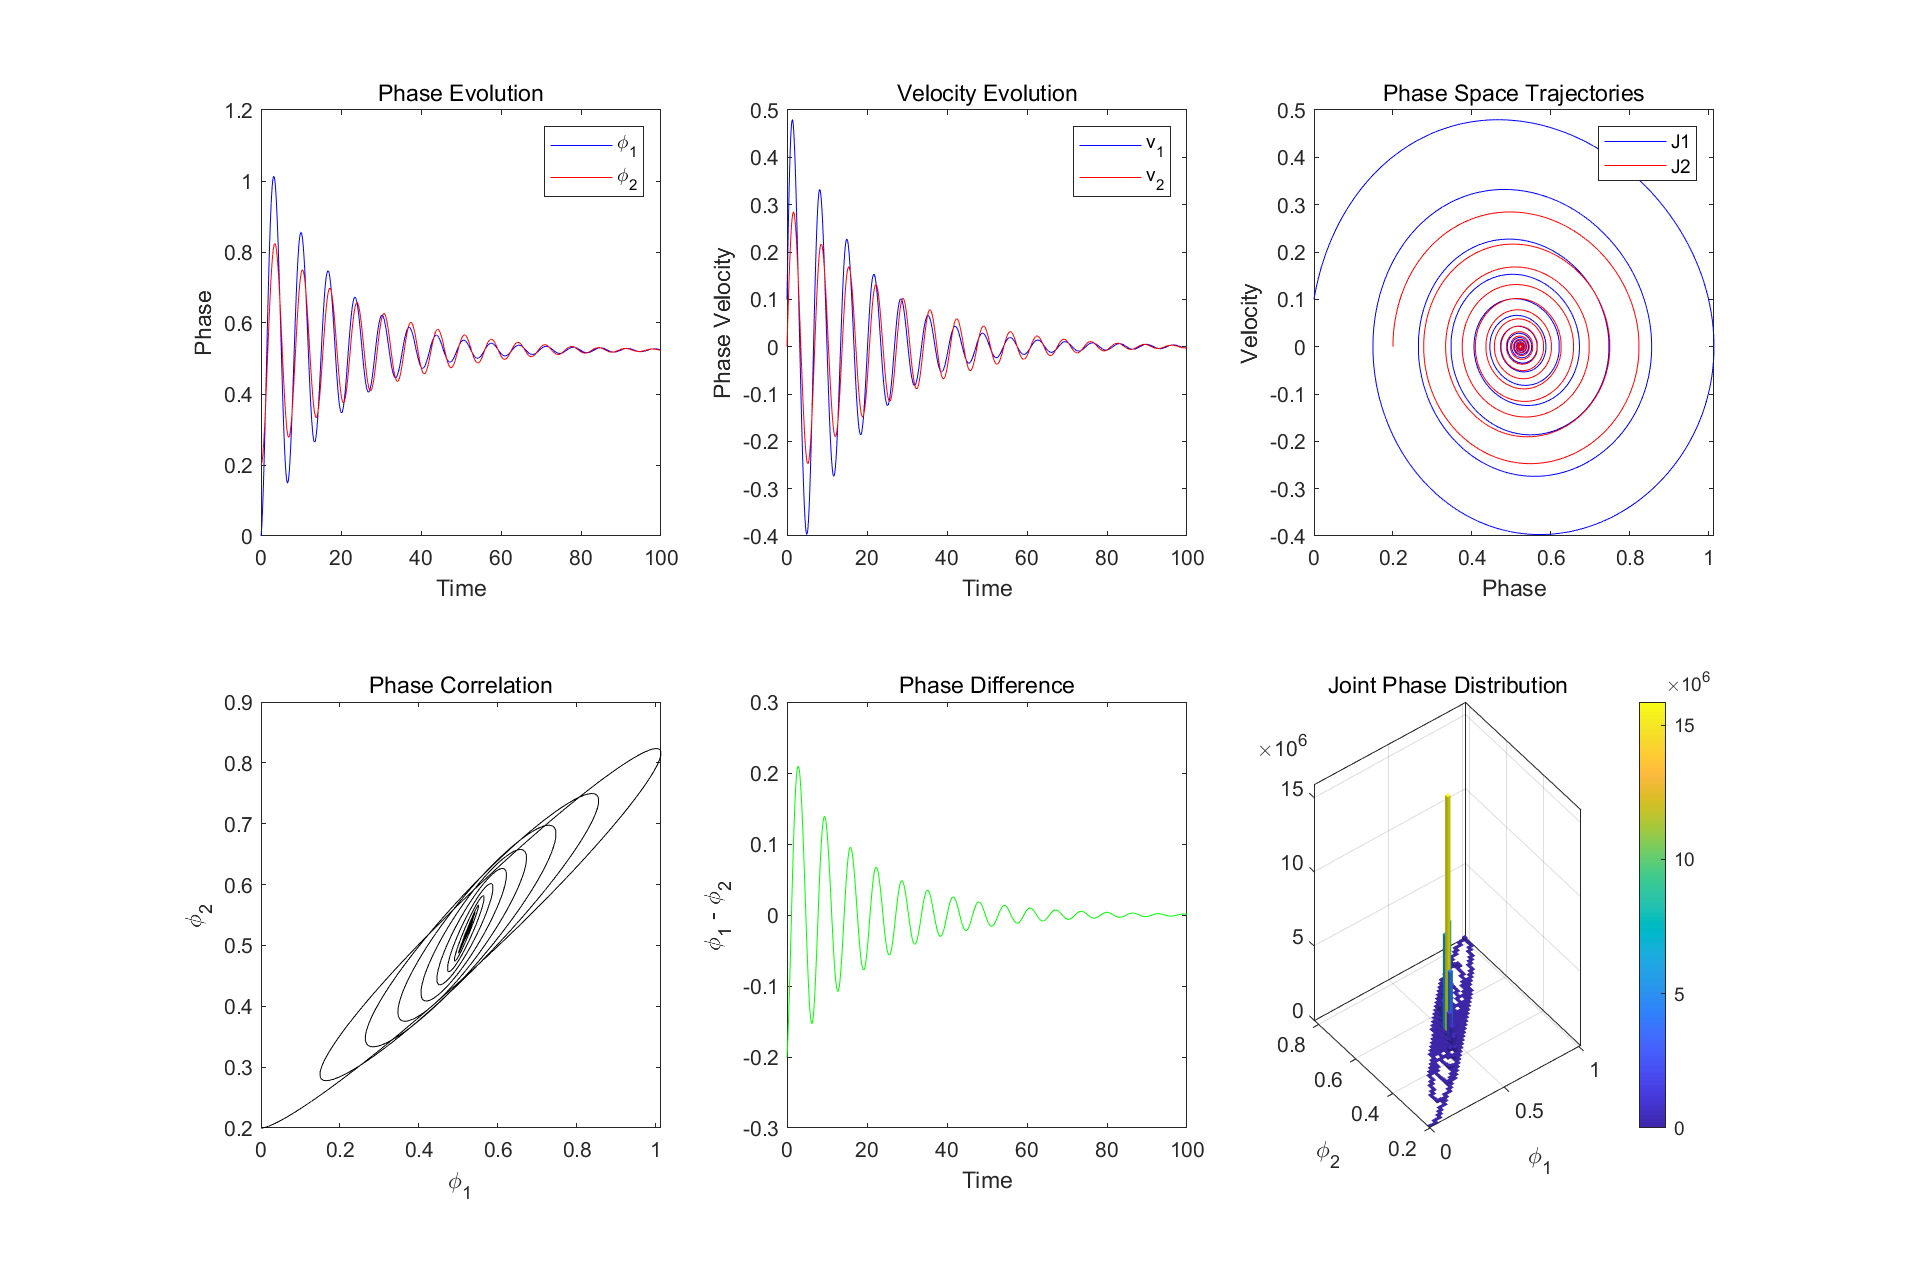
\includegraphics[width=6in]{PhaseSpace.eps}
    \end{minipage}
  \end{center}
  \caption{Analyze phase space dynamics with $\beta_{J_i}=0.1$, $i_{c_i}=0.8$, $\kappa_i=0.05$ and  $\sigma_i=0.01, i=1, 2$.}
\end{figure}
Now we add noise terms. We'll use Euler-Maruyama method for SDEs. We rewrite the system \eqref{n1}-\eqref{n2} as
\begin{align*}
 d\phi_1&=v_1dt,\\
           dv_1&=[i_1-\beta_{J_1}v_1-\sin(\phi_1)+\kappa_1(\phi_2-\phi_1)]dt+\sigma_1dW_1,  \\
 d\phi_2&=v_2dt,\\
dtv_2&=[i_2-\beta_{J_2}v_2-\sin(\phi_2)+\kappa_2(\phi_1-\phi_2)]dt+\sigma_2dW_2,
\end{align*}
where $W_1$ and $W_2$ are independent white noises, and $\sigma_1, \sigma_2$ are noise intensities related to the thermal noise.
We assume the fluctuation-dissipation relation, so the noise intensity is related to the damping and temperature. In normalized units, we can set $\sigma_i=\sqrt{2k_bT/R_i}, i=1, 2$ for temperature $T$ in normalized units.


\begin{figure}[H]
\begin{center}
\begin{minipage}{4in}
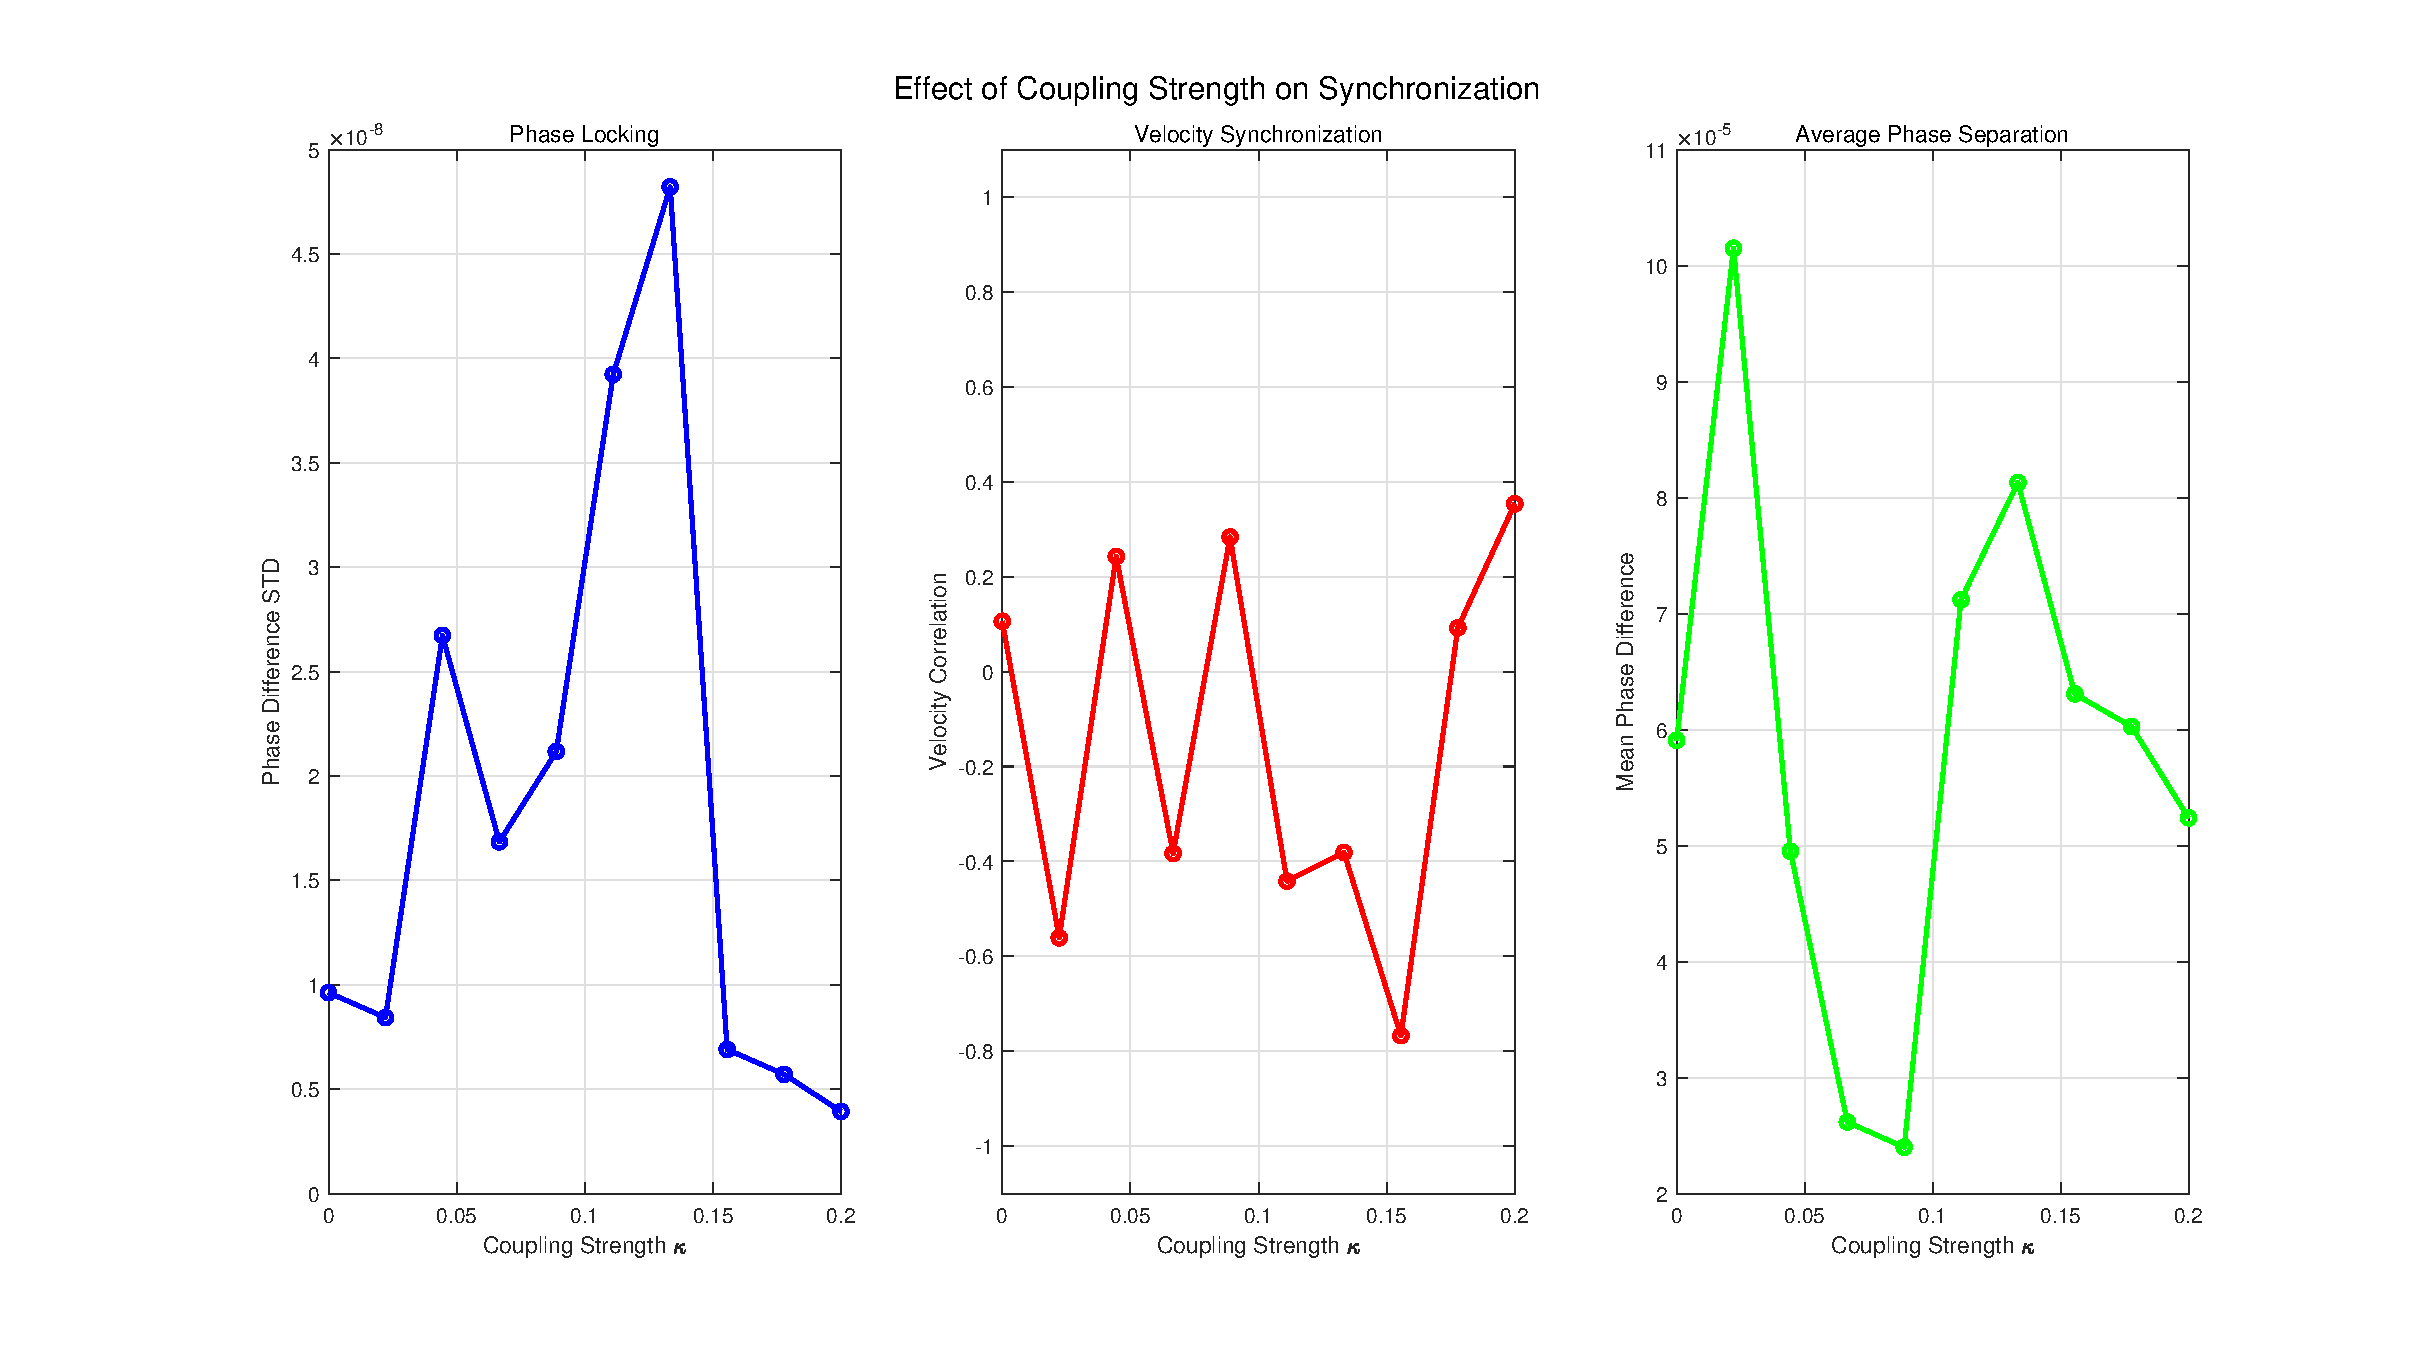
\includegraphics[width=4in]{CouplingStrength.eps}
\end{minipage}
\end{center}
\caption{Study effect of coupling strength on synchronization with $\beta_{J_i}=0.1$, $i_{c_i}=0.8$, and $\sigma_i=0.01, i=1, 2$.}
\end{figure}
\section{Sampling rare events}
Josephson junction systems exhibit important rare events:
\begin{enumerate}
  \item Phase slips (quantum tunneling between potential minima)
  \item Switching currents
  \item Synchronization transitions
\end{enumerate}
Score-based models excel at sampling from low-probability regions of the distribution, which is perfect for studying these rare but physically crucial events.

\textbf{Bifurcation analysis}: As the coupling parameters between Josephson junctions evolve, the score landscape learned by generative models undergoes profound qualitative transitions, revealing critical thresholds where the system's dynamics fundamentally reorganize. These bifurcations manifest as sudden changes in the preferred phase configurations, where weakly coupled junctions may transition from independent oscillations to phase-locked states, or from synchronous to chaotic regimes. The score function's topology--capturing the gradient of the log-probability distributio--serves as a sensitive detector of these emergent dynamical patterns, with its contours reshaping dramatically at critical coupling strengths. This allows for precise mapping of parameter regions where the system exhibits multistability, enabling the prediction of spontaneous symmetry breaking and the emergence of collective modes that are not apparent from individual junction dynamics alone.

\textbf{Noise-induced transitions}: Thermal noise plays a paradoxical role in facilitating transitions between metastable states that would otherwise be separated by insurmountable energy barriers in the deterministic limit. The score-based framework naturally captures how stochastic fluctuations enable rare but physically crucial events--such as phase slips and switching currents--by effectively lowering the activation energy required for state transitions. By learning the joint probability landscape of junction phases and velocities, generative models can quantify transition rates between metastable basins and reveal how noise correlation times and amplitudes influence synchronization stability. This approach provides deep insights into the fundamental trade-offs between noise resilience and sensitivity in quantum circuits, demonstrating how carefully engineered noise can actually enhance certain quantum information processing tasks while degrading others.




\section{Parameter inference}
We could learn the inverse mapping: from observed dynamics $(\phi_1(t),\phi_2(t))$
to underlying parameters $(\beta_{J_1},\beta_{J_2},\kappa_1,\kappa_2)$.




\section{Conclusions and future challenges}

\textbf{Multi-junction generalization}: Extending this analysis to larger junction arrays unveils rich emergent synchronization phenomena that transcend pairwise coupling effects. As the system size increases, the score landscape evolves to capture collective behaviors such as chimera states (where synchronous and asynchronous populations coexist), frustration in geometrically constrained arrays, and the spontaneous emergence of topological defects in phase ordering. The generative modeling approach scales naturally to high-dimensional state spaces, learning the complex correlations that give rise to macroscopic coherence from microscopic interactions. This framework enables the discovery of novel dynamical phases in quantum circuit networks and provides powerful design principles for optimizing synchronization in large-scale quantum processors, where emergent phenomena can either enhance computational capabilities or introduce destructive collective noise that must be carefully mitigated.


\begin{thebibliography}{00}
\bibitem{Y}
S. Yuan, Stochastic dynamics of the resistively shunted superconducting tunnel junction system under the impact of thermal fluctuations, \emph{Chaos, Solitons and Fractals},
2025, 199: 116917.


\end{thebibliography}



\end{document}

\endinput
%%
%% End of file `elsarticle-template-num-names.tex'.
